\documentclass[a4paper,11pt,oneside,openany]{memoir}

\usepackage{fontspec}
\usepackage{amsmath} % a pretty standard package to enlarge your inventory of symbols
\usepackage{amssymb} % another common package for symbols
\usepackage[hidelinks]{hyperref} % enables hyperlinks in your document (no worries -- they show up only on the screen. When you print a hard copy, the colored boxes aren't there)
\usepackage{url} % helps typeset URLs properly, typically with the command \url
\usepackage[margin=.75in]{geometry} % page layout
\usepackage{tikz}
\usepackage{tikz-qtree}
\usepackage{wrapfig}
%\usepackage{subcaption}
\usepackage{booktabs} % creates beautiful and professional tables
\usepackage{multicol}
\usepackage{multirow}
\usepackage{textcomp}
\usepackage{expex}
\usepackage{enumitem}
\usepackage{tablefootnote}
\usepackage[calc,english]{datetime2}
\usepackage{suffix}
\usepackage{afterpage}
\usepackage{bookmark}
\usepackage{blindtext}
\usepackage{phonrule}
\usepackage[glosses,indexonlyfirst,nonumberlist,toc,nomain,mcolblock,,nogroupskip]{leipzig}
\usepackage{etoolbox}

\setmainfont{Brill}

%---generic symbols---%
\newcommand{\dao}{$\to$}
\newcommand{\nm}{\symbol{"2205}}
\newcommand{\ra}{\textgreater}
\newcommand{\ipkt}{·}
\newcommand{\til}{\textasciitilde}
\newcommand{\langbr}{⟨}
\newcommand{\rangbr}{⟩}

\newcommand{\ortho}[1]{$\langle$#1$\rangle$}
\newcommand{\bripa}[1]{[#1]}
\newcommand{\phipa}[1]{/#1/}
\newcommand{\eng}[1]{`#1'}

%---IPA---%
%consonants
\newcommand{\bilaf}{ɸ}
\newcommand{\bilav}{β}
\newcommand{\tht}{θ}
\newcommand{\labrox}{ʋ}
\newcommand{\latfric}{ɬ}
\newcommand{\latfrivoic}{ɮ}
\newcommand{\darkl}{ɫ}
\newcommand{\alvr}{ɹ}
\newcommand{\alvrap}{ɾ}
\newcommand{\alvlap}{ɺ}
\newcommand{\esh}{ʃ}
\newcommand{\ezh}{ʒ}
\newcommand{\alvpalesh}{ɕ}
\newcommand{\alvpalezh}{ʑ}
\newcommand{\paljstop}{ɟ}
\newcommand{\paljfric}{ʝ}
\newcommand{\egna}{ɲ}
\newcommand{\retesh}{ʂ}
\newcommand{\retezh}{ʐ}
\newcommand{\retna}{ɳ}
\newcommand{\egh}{ɣ}
\newcommand{\engma}{ŋ}
\newcommand{\vell}{ʟ}
\newcommand{\velr}{ʁ}
\newcommand{\velprox}{ɰ}
\newcommand{\uvux}{χ}
\newcommand{\pharox}{ʕ}
\newcommand{\glotstop}{ʔ}
%vowels
\newcommand{\frno}{ø}
\newcommand{\bari}{ɨ}
\newcommand{\unru}{ɯ}
\newcommand{\unro}{ɤ}
\newcommand{\eps}{ɛ}
\newcommand{\oeps}{œ}
\newcommand{\sche}{ɘ}
\newcommand{\schwa}{ə}
\newcommand{\centruh}{ɜ}
\newcommand{\opno}{ɔ}
\newcommand{\aesh}{æ}
\newcommand{\oesh}{ɶ}
\newcommand{\centra}{ɐ}
\newcommand{\ahoh}{ɒ}
%diacritics and modifiers
\newcommand{\asp}{ʰ}
\newcommand{\lab}{ʷ}
\newcommand{\pal}{ʲ}
\newcommand{\jekt}{ʼ}
\newcommand{\nav}{̃}
\newcommand{\rhot}{˞}
\newcommand{\sylb}{̩}
\newcommand{\vless}{̥}
\newcommand{\upvless}{̊}
\newcommand{\bck}{̠}
\newcommand{\dwnwrd}{̞}
\newcommand{\upwrd}{̝}
\newcommand{\lamino}{̻}
\newcommand{\apico}{̺}
\newcommand{\lowap}{̞}
\newcommand{\prstr}{ˈ}
\newcommand{\scstr}{ˌ}
\newcommand{\tiebar}{͡}
\newcommand{\lgth}{ː}
\newcommand{\linglab}{̼}
%tone letters
\newcommand{\toneH}{˥}
\newcommand{\toneM}{˧}
\newcommand{\toneL}{˩}
\newcommand{\toneMH}{˦}
\newcommand{\toneML}{˨}

\definelingstyle{default}{glstyle=nlevel,numoffset=3em,textoffset=1.5em,exskip=.75ex,belowglpreambleskip=.25ex,aboveglftskip=.25ex,everyglft=\it}

\lingset{lingstyle=default}

\DTMnewdatestyle{eurodate}{%
    \renewcommand{\DTMdisplaydate}[4]{%
        \number##3.\nobreakspace%           day
        \DTMmonthname{##2}\nobreakspace%    month
        \number##1%                         year
    }%
    \renewcommand{\DTMDisplaydate}{\DTMdisplaydate}%
}

\DTMsetdatestyle{eurodate}

%----------------------------
%---------Glossaries---------
%----------------------------

\makenoidxglossaries

\newleipzig{test}{tst}{It's a test!}

\glssetwidest{CABBA}

\makeatletter
\newglossarystyle{fixed-mcols}{%
    \setglossarystyle{alttree}%
    \renewenvironment{theglossary}%
    {%
        \begin{multicols}{3}%
            \def\@gls@prevlevel{-1}%
%           \mbox{}\par
        }%
        {\par\end{multicols}}%
}
\makeatother

%---------------------------
%---------------------------

\newcommand{\enl}[1]{\textit{#1}}
\newcommand{\enlq}[1]{«~#1»}
\newcommand{\proto}[1]{\textit{*#1}}

%---Lang Romanization---%
%\newcommand{\ph}{φ}
%\newcommand{\te}{ϑ}
%\newcommand{\kh}{χ}
\newcommand{\ppa}{π}
\newcommand{\tta}{τ}
\newcommand{\kka}{κ}
\newcommand{\engga}{ng}
\newcommand{\Ppa}{Π}
\newcommand{\Tta}{Τ'}
\newcommand{\Kka}{Κ'}
\newcommand{\Engga}{Ng}

\newcommand{\suph}{$^\textsc{h}$}
\newcommand{\supglot}{$^\textsc{\glotstop}$}
\newcommand{\supho}{$^{\textsc{h}_{o}}$}
\newcommand{\supgloto}{$^{\textsc{\glotstop}_{o}}$}
\newcommand{\supha}{$^{\textsc{h}_{a}}$}
\newcommand{\supglota}{$^{\textsc{\glotstop}_{a}}$}
\newcommand{\suphi}{$^{\textsc{h}_{i}}$}
\newcommand{\supgloti}{$^{\textsc{\glotstop}_{i}}$}

\newcommand{\parentlang}{Enłalen}
\newcommand{\childlangone}{Daughterlang}
\newcommand{\childlangtwo}{Sonlang}
\newcommand{\childlangthree}{Kidlang}

\newlength{\drop}% for my convenience
\newcommand*{\titleP}{\begingroup%
%\FSfont{5bo} % FontSite Bergamo (Bembo)
\drop = 0.12\textheight
\vspace*{\drop}
\begin{center}
{\huge A Grammar of}\\[\baselineskip]
{\HUGE\sc \parentlang}\par
\end{center}
\vspace*{3\drop}
{\large By {\sc Bethany E. Toma}}
\vfill
{\today}
\vspace*{0.5\drop}
\endgroup}

\maxsecnumdepth{section}
\maxtocdepth{subsection}
\cftsetindents{subsection}{5em}{0em}

\setlength{\parindent}{0pt}
\nonzeroparskip

\preto{\backmatter}{\addtocontents{toc}{\protect\addvspace{16pt}}}

\begin{document}

\begin{titlingpage}
\titleP
%\clearpage
\end{titlingpage}
\frontmatter

\chapter{Background \& Motivation}

The languages documented herein are constructed languages (aka `conlangs') developed solely for the purposes of my own artistic fulfullment. This type of conlang is generally called an `artlang' within conlanging circles. These conlangs belong to a constructed universe (aka `conworld') of my own making. Much like famous author and conlanger J.R.R. Tolkien, I developed a conworld primarily as a place to ground my conlangs and place their fictional `speakers,' rather than primarily building a conworld and creating conlangs for the secondary purpose of `fleshing it out.' For me, conlanging itself is a joy and the artistic endeavor I truly wish to dedicate my time to. Unlike Tolkien, I have not fleshed my conworld out with much detail as of yet. I hope to add more details about this conworld here in the future. For now, I assert to the reader that the languages documented within this book are entirely fictional and that my goals in creating them have been entirely for my own enjoyment and artistic fulfillment.

\clearpage
\tableofcontents

\setglossarystyle{fixed-mcols}

\printnoidxglossary[type=\leipzigtype,title={Glossing Abbreviations}]

\mainmatter

\part{\parentlang{}}

\documentclass[a4paper,11pt,oneside,openany]{memoir}

\usepackage{fontspec}
\usepackage{amsmath} % a pretty standard package to enlarge your inventory of symbols
\usepackage{amssymb} % another common package for symbols
\usepackage[hidelinks]{hyperref} % enables hyperlinks in your document (no worries -- they show up only on the screen. When you print a hard copy, the colored boxes aren't there)
\usepackage{url} % helps typeset URLs properly, typically with the command \url
\usepackage[margin=.75in]{geometry} % page layout
\usepackage{tikz}
\usepackage{tikz-qtree}
\usepackage{wrapfig}
%\usepackage{subcaption}
\usepackage{booktabs} % creates beautiful and professional tables
\usepackage{multicol}
\usepackage{multirow}
\usepackage{textcomp}
\usepackage{expex}
\usepackage{enumitem}
\usepackage{tablefootnote}
\usepackage[calc,english]{datetime2}
\usepackage{suffix}
\usepackage{afterpage}
\usepackage{bookmark}
\usepackage{blindtext}
\usepackage{phonrule}
\usepackage[glosses,indexonlyfirst,nonumberlist,toc,nomain,mcolblock,,nogroupskip]{leipzig}
\usepackage{etoolbox}

\setmainfont{Brill}

%---generic symbols---%
\newcommand{\dao}{$\to$}
\newcommand{\nm}{\symbol{"2205}}
\newcommand{\ra}{\textgreater}
\newcommand{\ipkt}{·}
\newcommand{\til}{\textasciitilde}
\newcommand{\langbr}{⟨}
\newcommand{\rangbr}{⟩}

\newcommand{\ortho}[1]{$\langle$#1$\rangle$}
\newcommand{\bripa}[1]{[#1]}
\newcommand{\phipa}[1]{/#1/}
\newcommand{\eng}[1]{`#1'}

%---IPA---%
%consonants
\newcommand{\bilaf}{ɸ}
\newcommand{\bilav}{β}
\newcommand{\tht}{θ}
\newcommand{\labrox}{ʋ}
\newcommand{\latfric}{ɬ}
\newcommand{\latfrivoic}{ɮ}
\newcommand{\darkl}{ɫ}
\newcommand{\alvr}{ɹ}
\newcommand{\alvrap}{ɾ}
\newcommand{\alvlap}{ɺ}
\newcommand{\esh}{ʃ}
\newcommand{\ezh}{ʒ}
\newcommand{\alvpalesh}{ɕ}
\newcommand{\alvpalezh}{ʑ}
\newcommand{\paljstop}{ɟ}
\newcommand{\paljfric}{ʝ}
\newcommand{\egna}{ɲ}
\newcommand{\retesh}{ʂ}
\newcommand{\retezh}{ʐ}
\newcommand{\retna}{ɳ}
\newcommand{\egh}{ɣ}
\newcommand{\engma}{ŋ}
\newcommand{\vell}{ʟ}
\newcommand{\velr}{ʁ}
\newcommand{\velprox}{ɰ}
\newcommand{\uvux}{χ}
\newcommand{\pharox}{ʕ}
\newcommand{\glotstop}{ʔ}
%vowels
\newcommand{\frno}{ø}
\newcommand{\bari}{ɨ}
\newcommand{\unru}{ɯ}
\newcommand{\unro}{ɤ}
\newcommand{\eps}{ɛ}
\newcommand{\oeps}{œ}
\newcommand{\sche}{ɘ}
\newcommand{\schwa}{ə}
\newcommand{\centruh}{ɜ}
\newcommand{\opno}{ɔ}
\newcommand{\aesh}{æ}
\newcommand{\oesh}{ɶ}
\newcommand{\centra}{ɐ}
\newcommand{\ahoh}{ɒ}
%diacritics and modifiers
\newcommand{\asp}{ʰ}
\newcommand{\lab}{ʷ}
\newcommand{\pal}{ʲ}
\newcommand{\jekt}{ʼ}
\newcommand{\nav}{̃}
\newcommand{\rhot}{˞}
\newcommand{\sylb}{̩}
\newcommand{\vless}{̥}
\newcommand{\upvless}{̊}
\newcommand{\bck}{̠}
\newcommand{\dwnwrd}{̞}
\newcommand{\upwrd}{̝}
\newcommand{\lamino}{̻}
\newcommand{\apico}{̺}
\newcommand{\lowap}{̞}
\newcommand{\prstr}{ˈ}
\newcommand{\scstr}{ˌ}
\newcommand{\tiebar}{͡}
\newcommand{\lgth}{ː}
\newcommand{\linglab}{̼}
%tone letters
\newcommand{\toneH}{˥}
\newcommand{\toneM}{˧}
\newcommand{\toneL}{˩}
\newcommand{\toneMH}{˦}
\newcommand{\toneML}{˨}

\definelingstyle{default}{glstyle=nlevel,numoffset=3em,textoffset=1.5em,exskip=.75ex,belowglpreambleskip=.25ex,aboveglftskip=.25ex,everyglft=\it}

\lingset{lingstyle=default}

\DTMnewdatestyle{eurodate}{%
    \renewcommand{\DTMdisplaydate}[4]{%
        \number##3.\nobreakspace%           day
        \DTMmonthname{##2}\nobreakspace%    month
        \number##1%                         year
    }%
    \renewcommand{\DTMDisplaydate}{\DTMdisplaydate}%
}

\DTMsetdatestyle{eurodate}

%-----DICT COMMANDS------
%------------------------

\makeatletter
\@beginparpenalty=10000
\makeatother

\newcounter{dictwordcount}
\newcounter{definition}

\newenvironment{entrylist}{
    \begin{description}[leftmargin=*]
    }{
    \end{description}
    }

\makeatletter
\newenvironment{simplentry}[1]%
    {%
    \item[#1]\hfill
    \protected@edef\@currentlabelname{#1}%
    \setcounter{definition}{0}%
    \begin{description}[align=right,labelwidth=*,font=\normalfont]
    }{%
    \end{description}
    }%
\makeatother

\makeatletter
\newenvironment{dictentry}[3][]%
    {%
    \item[#2]\ifthenelse{\isempty{#1}}{\hfill}{\:\bripa{#1}\hfill}\\
    {\footnotesize #3}
    \protected@edef\@currentlabelname{#2}%
    \setcounter{definition}{0}%
    \refstepcounter{dictwordcount}%
    \begin{description}[align=right,labelwidth=*,font=\normalfont]
    }{%
    \end{description}
    }%
\makeatother

\newenvironment{entrysublist}{
    \vspace{2ex}
    \item[]\textit{Compounds \& Phrasal Forms}
    \begin{entrylist}
        \small
    }{
    \end{entrylist}
    }

\newcommand{\dictdef}[2][]{\refstepcounter{definition}%
    \item[\thedefinition.] \ifthenelse{\isempty{#1}}{
        #2
    }{
        \textit{#1}\: #2
    }%
    }%

\WithSuffix\newcommand\dictdef*[2][]{%
    \item[] \ifthenelse{\isempty{#1}}{
        #2
    }{
        \textit{#1} #2
    }%
    }

\newcounter{protwordcount}

\makeatletter
\newenvironment{protentry}[1]%
    {%
    \item[\proto{#1}]\hfill
    \protected@edef\@currentlabelname{#1}%
    \setcounter{definition}{0}%
    \refstepcounter{protwordcount}%
    \begin{description}[align=right,labelwidth=*,font=\normalfont]
    }{%
    \end{description}
    }%
\makeatother

%----------------------------
%---------Glossaries---------
%----------------------------

\makenoidxglossaries

\newleipzig{test}{tst}{It's a test!}

\glssetwidest{CABBA}

\makeatletter
\newglossarystyle{fixed-mcols}{%
    \setglossarystyle{alttree}%
    \renewenvironment{theglossary}%
    {%
        \begin{multicols}{3}%
            \def\@gls@prevlevel{-1}%
%           \mbox{}\par
        }%
        {\par\end{multicols}}%
}
\makeatother

%---------------------------
%---------------------------

\newcommand{\enl}[1]{\textit{#1}}
\newcommand{\enlq}[1]{«~#1»}
\newcommand{\proto}[1]{\textit{*#1}}

%---Lang Romanization---%
%\newcommand{\ph}{φ}
%\newcommand{\te}{ϑ}
%\newcommand{\kh}{χ}
\newcommand{\ppa}{π}
\newcommand{\tta}{τ}
\newcommand{\kka}{κ}
\newcommand{\engga}{ng}
\newcommand{\Ppa}{Π}
\newcommand{\Tta}{Τ'}
\newcommand{\Kka}{Κ'}
\newcommand{\Engga}{Ng}

\newcommand{\suph}{$^\textsc{h}$}
\newcommand{\supglot}{$^\textsc{\glotstop}$}
\newcommand{\supho}{$^{\textsc{h}_{o}}$}
\newcommand{\supgloto}{$^{\textsc{\glotstop}_{o}}$}
\newcommand{\supha}{$^{\textsc{h}_{a}}$}
\newcommand{\supglota}{$^{\textsc{\glotstop}_{a}}$}
\newcommand{\suphi}{$^{\textsc{h}_{i}}$}
\newcommand{\supgloti}{$^{\textsc{\glotstop}_{i}}$}

\newcommand{\parentlang}{Enłalen}
\newcommand{\childlangone}{Daughterlang}
\newcommand{\childlangtwo}{Sonlang}
\newcommand{\childlangthree}{Kidlang}

\newlength{\drop}% for my convenience
\newcommand*{\titleP}{\begingroup%
%\FSfont{5bo} % FontSite Bergamo (Bembo)
\drop = 0.12\textheight
\vspace*{\drop}
\begin{center}
{\huge A Grammar of}\\[\baselineskip]
{\HUGE\sc \parentlang}\par
\end{center}
\vspace*{3\drop}
{\large By {\sc Bethany E. Toma}}
\vfill
{\today}
\vspace*{0.5\drop}
\endgroup}

\maxsecnumdepth{section}

\setlength{\parindent}{0pt}
\nonzeroparskip

\begin{document}

\begin{titlingpage}
\titleP
%\clearpage
\end{titlingpage}
\frontmatter

\chapter{Background \& Motivation}
\clearpage
\tableofcontents

\setglossarystyle{fixed-mcols}

\printnoidxglossary[type=\leipzigtype,title={Glossing Abbreviations}]

\mainmatter

\part{\parentlang{} Grammar}

\chapter{Context \& Culture}

\Blindtext[2]

\ex
\begingl
\glpreamble
`Yesterday, I saw the dog and the cat fighting, and then...
\endpreamble
I[\Fsg]
example[example]
be[\Spl]
ah[\Acc]
\glft ...the dog hit the cat.'
\endgl
\xe

\Blindtext[3]

\pex
\a
\begingl
\glpreamble
`Yesterday, I saw the dog and the cat fighting, and then...
\endpreamble
I[\Fsg]
a\l k[dog]
\glft ...the dog hit the cat.'
\endgl
\a 
\begingl
\glpreamble
`I told my dog to stay, but then when I turned around...
\endpreamble
a\l k[dog]
hit[\Sarg]
\glft ...the dog hit the cat.'
\endgl
\xe

\Blindtext[1]

\chapter{Phonology}

\section{Phonemics \& Allophony}

\subsection{Phoneme Inventory}

\begin{table}[h]
    \centering
    \begin{tabular}{@{}rccc@{}}
    \toprule
     & Labial & Coronal & Velar \\ \midrule
    Ejective & pʼ & tʼ & kʼ \\
    Plosive & p & t & k \\
    Fricative & f & s & \\
    Nasal & m & n & ŋ \\
    Liquid &  & l & ʟ \\ \bottomrule
    \end{tabular}
    \caption{Consonant Inventory}
    \label{tab:enl-consonants}
\end{table}

\begin{table}[h]
    \centering
    \begin{tabular}{@{}rccc@{}}
    \toprule
    \multicolumn{1}{l}{} & Front & Central & Back \\ \midrule
    High & i j &  &  \\
    Mid &  &  & o w \\
    Low &  & a \pharox\dwnwrd &  \\ \bottomrule
    \end{tabular}
    \caption{Vowel \& Glide Inventory}
    \label{tab:enl-vowels}
\end{table}

\parentlang{} possesses the glides \bripa{j, w, \pharox\dwnwrd} in certain positions, but these are analyzed as consonantal allophones of the vowel phonemes.

\subsection{Allophony \& Phonotactics}

To be replaced with better versions of these and such later:

\begin{itemize}
    \item Vowels \phipa{i, o, a} become nasal \bripa{e\nav, o\nav, a\nav} when they precede a nasal
    \item \phipa{l} becomes \bripa{\vell} before a velar consonant and \bripa{\bilav\dwnwrd} before a labial consonant. \phipa{w} is considered velar for these purposes.
    \item \phipa{\vell} becomes \bripa{\darkl} before a coronal consonant and \bripa{w} before a labial consonant. \phipa{w} is considered velar for these purposes.
    \item Front vowels and semivowels \bripa{i, e\nav, j} become central \bripa{\bari, \sche\nav, j} before non-palatal dorsal sonorants (including vowels) \bripa{\engma, \vell, w, \pharox\dwnwrd, a} and after non-palatal dorsal obstruents \bripa{k, k\jekt}
    \item Back vowel \bripa{o} becomes central \bripa{\sche} before \bripa{j, i(\lgth)}
    \item Mid, non-front vowels \bripa{\sche, \sche\nav, o, o\nav} become high \bripa{\bari, \bari\nav, u, u\nav} after a high semivowel \bripa{j, w, \velprox}
    \item Mid vowels \bripa{o, o\nav, e\nav, \sche, \sche\nav} become low lax \bripa{\ahoh, \ahoh\nav, \aesh\nav, a, a\nav} before non-palatal dorsal sonorants (\emph{not} including vowels) \bripa{\engma, \vell, w, \pharox\dwnwrd} and after non-palatal dorsal obstruents \bripa{k, k\jekt}.
    \item Nasals assimilate in place-of-articulation to a following obstruent.
    \item In Northern lects only:
    \begin{itemize}
        \item Standalone fricatives become debuccalized to \bripa{h} intervocalically. Geminate fricatives become single fricatives.
        \item Standalone voiceless stops become voiceless fricatives intervocalically. Geminate voiceless stops become single voiceless stops.
        \item Standalone ejectives become unaspirated voiceless stops intervocalically. Geminate ejectives become single ejectives.
    \end{itemize}
    \item In Southern lects only:
    \begin{itemize}
        \item Standalone voiceless fricatives become voiced intervocalically. Geminate voiceless fricatives become single voiceless fricatives.
        \item Standalone voiceless stops become voiced stops intervocalically. Geminate voiceless stops become single voiceless stops.
        \item Geminate ejectives become single ejectives. Standalone ejectives remain the same intervocalically.
    \end{itemize}
\end{itemize}

\section{Structure \& Suprasegmental Features}

\subsection{Syllable Structure}

\subsection{Stress}

%Stress in \parentlang{} is weight-sensitive, relying on a principle that classifies syllables containing long vowels as `heavy' and those without long vowels as `light.' Note that this is only the case for the stem---peripherals are considered light even when the nucleus is a long vowel. The determination of stress location is unbounded, so stress may appear anywhere in a given word, with right-headed assignment for heavy syllables and left-headed assignment for light syllables. The result of this is that stress is placed on the rightmost heavy syllable if there is one, or on the first syllable if there are none.

\subsection{Tone}

\section{Prosody}

\section{Transcription}

Enłalen's `romanization', used only for documentation purposes, is generally an unremarkable representation of the IPA-phonology, with a few exceptions:
\begin{itemize}
    \item \phipa{j} is written as \ortho{y}
    \item \phipa{\pharox\dwnwrd} is written as \ortho{r}
    \item \phipa{\vell} is written as \ortho{ł}
    \item \phipa{i} is written as \ortho{i} in most positions, but is written with \ortho{e} when it precedes a nasal and is realized as \bripa{ẽ}. Nasalization is not otherwise illustrated in the orthography.
    \item \phipa{\engma} is written as \ortho{n} in contexts in which it does not contrast with \phipa{n} (i.e., when it precedes velar phones as in \enl{enłalen} \bripa{ẽŋ\vell alẽn}) but is written as \ortho{\engga} in positions in which it contrasts with \phipa{n} (as in \enl{ale\engga} \bripa{alẽ\engma}).
    \item The ejective series \phipa{p\jekt{} t\jekt{} k\jekt{}} is written with the letters \ortho{\ppa{} \tta{} \kka{}}
    \item Phonemic high tone on a syllable is indicated by placing the acute diacritic on the vowel of that syllable, and phonemic low tone on a syllable is indicated by placing an underdot diacritic on the vowel of that syllable.
\end{itemize}

\section{Orthography}

write this later.


\chapter{Morphology}

\section{Historical Morphophonology}

\subsection{Metrical categories}

Each root in \parentlang{} can be classified into one of five categories based on the sequence of phonemic long and short vowels in its form in Old Elvish. In \parentlang{}, these categories are named for the metrical styles of Old Elvish poetry; in English, we thus use terms for different types of metrical feet from Greek poetry. As such, the categories are as follows:
\begin{description}[labelindent=30pt,leftmargin=*,rightmargin=30pt]
    \item[Iambic:] Old Elv. root ends with a long vowel, with a short vowel in the preceding syllable. If the original root contains at least three syllables, the antepenult vowel is long.
    \item[Anapaestic:] Old Elv. root ends with a long vowel, with short vowels in the preceding two syllables. Words formed from Old Elvish roots that contain only a single syllable with a long vowel are also generally categorized as anapaestic.
    \item[Dactylic:] Old Elv. root ends with a short vowel preceded by another short vowel
    \item[Trochaic:] Old Elv. root ends with a short vowel preceded by a long vowel. If the root contains at least four syllables, the fourth-to-last and antepenult vowel form another long-short trochee pattern
    \item[Quasi-trochaic:] Old Elv. root ends with a short vowel preceded by a long vowel, preceded by two short vowels. Quasi-trochaic roots only occur when a root contains at least four syllables.
\end{description}

These categorizations matter for \parentlang{} because the final metrical pattern of a root affected the realization of the metrical patterns of affixes, resulting in affixes having different forms depending on the preceding metrical patterns. Further complicating matters is the fact that these affixes are applied sequentially and the application of a given affix can (and usually does) change a word's metrical category.

Based on its own length and phonemic metrical pattern in Old Elvish, a given affix can fall into one of nine categories:
\begin{description}[labelindent=30pt,leftmargin=*,rightmargin=30pt]
    \item[Short:] consisted of a single syllable with a short vowel in Old Elvish. Iambic roots become trochaic, dactylic roots become anapaestic, trochaic and quasi-trochaic roots become dactylic, and anapaestic roots become quasi-trochaic \emph{unless} they consisted only of a single long-vowelled syllable in Old Elvish, in which case they become trochaic.
    \begin{center}
    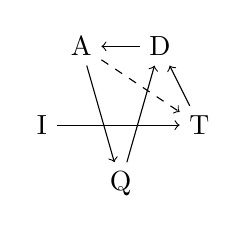
\begin{tikzpicture}
        \node[] at (-0.5,0.75) (a) {A};
        \node[] at (1,-0.25) (t) {T};
        \node[] at (0.5,0.75) (d) {D};
        \node[] at (-1,-0.25) (i) {I};
        \node[] at (0,-1) (q) {Q};
        \draw[->] (a) -- (q);
        \draw[dashed,->] (a) -- (t);
        \draw[->] (t) -- (d);
        \draw[->] (q) -- (d);
        \draw[->] (i) -- (t);
        \draw[->] (d) -- (a);
    \end{tikzpicture}
    \end{center}
    \item[Long:] consisted of a single syllable with a long vowel in Old Elvish. As with short affixes, iambic roots become trochaic, dactylic roots become anapaestic, anapaestic roots become quasi-trochaic or trochaic (under the same circumstances described above), \emph{but} trochaic and quasi-trochaic roots become iambic rather than dactylic.
    \begin{center}
        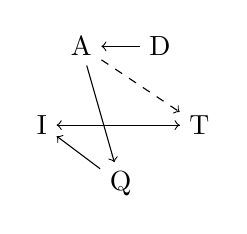
\begin{tikzpicture}
            \node[] at (-0.5,0.75) (a) {A};
            \node[] at (1,-0.25) (t) {T};
            \node[] at (0.5,0.75) (d) {D};
            \node[] at (-1,-0.25) (i) {I};
            \node[] at (0,-1) (q) {Q};
            \draw[->] (a) -- (q);
            \draw[dashed,->] (a) -- (t);
            \draw[->] (t) -- (i);
            \draw[->] (q) -- (i);
            \draw[->] (i) -- (t);
            \draw[->] (d) -- (a);
        \end{tikzpicture}
        \end{center}
    \item[Iambic:] consisted of two syllables, the latter with a long vowel and the former with a short vowel. Anapaestic roots become iambic, iambic roots become dactylic, dactylic roots become quasi-trochaic, and trochaic and quasi-trochaic roots remain trochaic and quasi-trochaic, respectively.
    \begin{center}
        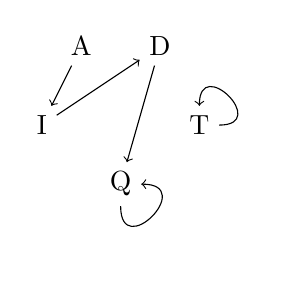
\begin{tikzpicture}
            \node[] at (-0.5,0.75) (a) {A};
            \node[] at (1,-0.25) (t) {T};
            \node[] at (0.5,0.75) (d) {D};
            \node[] at (-1,-0.25) (i) {I};
            \node[] at (0,-1) (q) {Q};
            \draw[->] (a) to (i);
            \draw[->] (t) to [out=0,in=90,loop,looseness=4.8] (t);
            \draw[->] (q) to [out=-90,in=0,loop,looseness=4.8] (q);
            \draw[->] (i) to (d);
            \draw[->] (d) to (q);
        \end{tikzpicture}
    \end{center}
    \item[Trochaic:] consisted of two syllables, the latter with a short vowel and the former with a long vowel. Anapaestic roots become dactylic, dactylic roots become quasi-trochaic, quasi-trochaic roots become trochaic, and iambic and trochaic roots remain iambic and trochaic, respectively.
    \begin{center}
        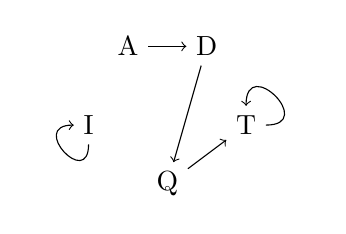
\begin{tikzpicture}
            \node[] at (-0.5,0.75) (a) {A};
            \node[] at (1,-0.25) (t) {T};
            \node[] at (0.5,0.75) (d) {D};
            \node[] at (-1,-0.25) (i) {I};
            \node[] at (0,-1) (q) {Q};
            \draw[->] (a) to (d);
            \draw[->] (t) to [out=0,in=90,loop,looseness=4.8] (t);
            \draw[->] (i) to [out=-90,in=180,loop,looseness=4.8] (i);
            \draw[->] (q) to (t);
            \draw[->] (d) to (q);
        \end{tikzpicture}
    \end{center}
    \item[Pyrrhic:] consisted of two syllables, both of which contained short vowels. Anapaestic and iambic roots become dactylic, dactylic roots become quasi-trochaic, quasi-trochaic roots become iambic, and trochaic roots remain trochaic.
    \begin{center}
        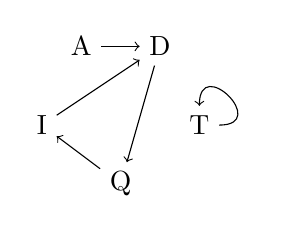
\begin{tikzpicture}
            \node[] at (-0.5,0.75) (a) {A};
            \node[] at (1,-0.25) (t) {T};
            \node[] at (0.5,0.75) (d) {D};
            \node[] at (-1,-0.25) (i) {I};
            \node[] at (0,-1) (q) {Q};
            \draw[->] (a) to (d);
            \draw[->] (t) to [out=0,in=90,loop,looseness=4.8] (t);
            \draw[->] (i) to (d);
            \draw[->] (q) to (i);
            \draw[->] (d) to (q);
        \end{tikzpicture}
    \end{center}
    \item[Anapaestic:] consisted of three syllables, the last of which was long with the prior two being short. Quasi-trochaic roots become trochaic, trochaic roots become dactylic, dactylic roots become iambic, iambic roots become anapaestic, and anapaestic roots remain anapaestic.
    \begin{center}
        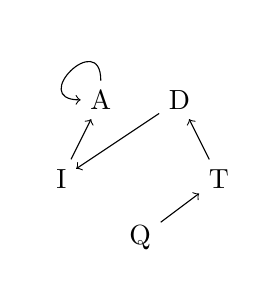
\begin{tikzpicture}
            \node[] at (-0.5,0.75) (a) {A};
            \node[] at (1,-0.25) (t) {T};
            \node[] at (0.5,0.75) (d) {D};
            \node[] at (-1,-0.25) (i) {I};
            \node[] at (0,-1) (q) {Q};
            \draw[->] (t) to (d);
            \draw[->] (a) to [out=90,in=180,loop,looseness=4.8] (a);
            \draw[->] (i) to (a);
            \draw[->] (q) to (t);
            \draw[->] (d) to (i);
        \end{tikzpicture}
    \end{center}
    \item[Amphibrachic:] consisted of three syllables, the middle of which was long with the other two being short. Dactylic roots remain dactylic. All other roots become or remain trochaic.
    \begin{center}
        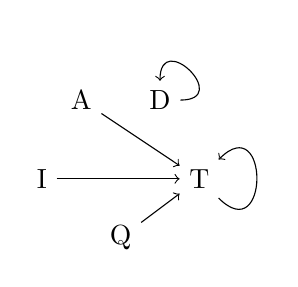
\begin{tikzpicture}
            \node[] at (-0.5,0.75) (a) {A};
            \node[] at (1,-0.25) (t) {T};
            \node[] at (0.5,0.75) (d) {D};
            \node[] at (-1,-0.25) (i) {I};
            \node[] at (0,-1) (q) {Q};
            \draw[->] (t) to [out=-45,in=45,loop,looseness=4.8] (t);
            \draw[->] (d) to [out=0,in=90,loop,looseness=4.8] (d);
            \draw[->] (i) to (t);
            \draw[->] (q) to (t);
            \draw[->] (a) to (t);
        \end{tikzpicture}
    \end{center}
    \item[Dactylic:] consisted of three syllables, the first of which was long with the other two being short. Anapaestic and iambic roots become trochaic. All other roots become or remain dactylic.
    \begin{center}
        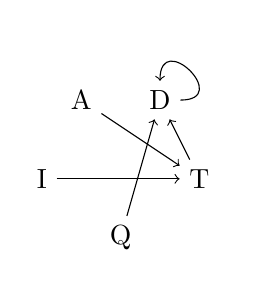
\begin{tikzpicture}
            \node[] at (-0.5,0.75) (a) {A};
            \node[] at (1,-0.25) (t) {T};
            \node[] at (0.5,0.75) (d) {D};
            \node[] at (-1,-0.25) (i) {I};
            \node[] at (0,-1) (q) {Q};
            \draw[->] (t) to (d);
            \draw[->] (d) to [out=0,in=90,loop,looseness=4.8] (d);
            \draw[->] (i) to (t);
            \draw[->] (q) to (d);
            \draw[->] (a) to (t);
        \end{tikzpicture}
    \end{center}
    \item[Cretic:] consisted of three syllables, the first and last of which were long and the middle of which was short. Iambic roots become trochaic, and anapaestic roots remain anapaestic. All other roots become iambic.
    \begin{center}
        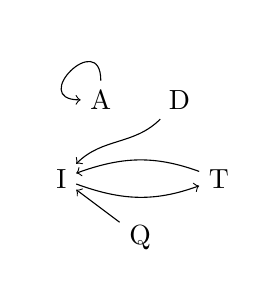
\begin{tikzpicture}
            \node[] at (-0.5,0.75) (a) {A};
            \node[] at (1,-0.25) (t) {T};
            \node[] at (0.5,0.75) (d) {D};
            \node[] at (-1,-0.25) (i) {I};
            \node[] at (0,-1) (q) {Q};
            \draw[->] (t) to [out=160,in=20] (i);
            \draw[->] (d) to [out=225,in=45] (i);
            \draw[->] (i) to [out=-20,in=200] (t);
            \draw[->] (q) to (i);
            \draw[->] (a) to [out=90,in=180,loop,looseness=4.8] (a);
        \end{tikzpicture}
    \end{center} 
\end{description}
While there may be some indicator of which category a given affix falls into based on how it patterns with roots, by and large these cannot be reliably inferred from surface forms without some knowledge of historical forms. Within this grammar, the underlying pattern of a given affix will be listed when relevant. 

Since affixes naturally appear differently in different environments, their differences will be listed when relevant. If in a context where pointing out each individual form is unnecessary or has already been done, the form used with anapaestic roots will be used as the citation form for nouns and the form used with dactylic roots will be used as the citation form for verbs.

\subsection{Historic glottals and vowels}

Sometimes a given affix form will be written out with a superscript \supho{} or \supglot{} preceding or following the affix. This indicates that in Old Elvish there was a historic \proto{h} or \proto{\glotstop} present at that boundary that could affect adjacent phones. When one of these is placed after an affix, a vowel is included as well to indicate what short vowel was present. These factors are listed to account for seemingly irregular behavior at morpheme boundaries.

For example, the form of the inclusive subject clitic that is placed after a dactylic root is \enl{-mạ\supho}, an iambic affix that turns the root quasi-trochaic. The form of the exclusive object clitic that is placed directly after is \enl{-\supglot wạ}. Without these morpheme-boundary indicators, one would expect the form to be \enl{-mạwạ}, but due to their interactions, it's actually \enl{-mạwwạ}. Minor `irregularities' like this frequently result from these interactions, which is why these superscript indicators are included when relevant.

\section{Nominal Morphology}

\section{Verbal Morphology}

\parentlang{} verbal morphology involves the use of affixes to mark tense as well as, in many contexts, using anaphoric clitics to indicate the person of verbal arguments. Tense affixes are mandatory and appear closest to the verb, whereas anaphoric clitics are only included in certain contexts and occur after any tense affix. Historically \parentlang{} possessed a negation affix that occurred even closer to the verb stem than tense marking; however, as negation is now largely indicated analytically, this is only apparent in the derivations of negation particles from \parentlang{} verbs.

\subsection{Tense Marking}



\subsection{Anaphoric Clitics}

\chapter{Syntax}

\chapter{Semantics}


%\part{\childlangone{} Grammar}

%\chapter{Context \& Culture}

%\chapter{Phonology}

%Daughterlang ideas to save for later:

% \begin{itemize}
%     \item \phipa{lw, \vell w} become \bripa{\alvr\lab, \velr\lab}
% \end{itemize}

% \subsection{Romanization}

% \chapter{Morphosyntax}

% \chapter{Semantics}

\part{Dictionary}

\setsecnumdepth{part}
\settocdepth{part}

\chapter{Old Elvish}

\begin{multicols*}{2}

\begin{entrylist}
    \begin{protentry}{hi\lgth lino}\label{OE:hiilino}
        \dictdef*{
            speech, talking, discussion, chatting, communication\\
            {\footnotesize Descendants: 
            \textit{\nameref{enl:enLalen_HLM}}
            }
        }
    \end{protentry}
    \begin{protentry}{hi\lgth na\glotstop ala\lgth}
    \label{OE:hiina7alaa}
        \dictdef*{
            the World, the physical realm, the mortal plane, this world\\
            {\footnotesize Descendants: 
            \textit{\nameref{enl:enLalen_HLM}}
            }
        }
    \end{protentry}
\end{entrylist}

\end{multicols*}

\chapter{En\l alen}

\begin{multicols*}{2}

\section{E}

\begin{entrylist}
    \begin{dictentry}[ẽ\engma\toneH\vell a\toneL lẽn\toneM]{énłạlen}{
        troch., from Old Elv. \proto{hi\lgth na\glotstop ala\lgth hili\lgth no} `World-speech' from \proto{\nameref{OE:hiina7alaa}} `the World' + \proto{\nameref{OE:hiilino}} `speech'
        }
        \label{enl:enLalen_HLM}
        \dictdef*[n.]{this language, En\l alen}
    \end{dictentry}
\end{entrylist}

\section{I}

\begin{entrylist}
    \begin{dictentry}[il\toneH jũn\toneM]{ílyon}{
        dacty., from Old Elv. \proto{\nameref{OE:hiilino}} `speech'
    }
        \dictdef*[v.]{
            utterance, statement, sentence
        }
        \begin{entrysublist}
            \begin{simplentry}{ẹn ílyon}
                \dictdef*[v.]{
                    to be sapient, to be intelligent, to be mentally aware, to have one's faculties (lit., to have speech)
                }
            \end{simplentry}
        \end{entrysublist}
    \end{dictentry}
\end{entrylist}

\end{multicols*}

\part{Texts \& Translations}

%\backmatter

\end{document}

\part{Old Elvish}


\chapter{Context}

\chapter{Phonology}

\chapter{Morphosyntax}


\backmatter

\setsecnumdepth{part}
\settocdepth{part}

\chapter{Old Elvish}

\begin{multicols*}{2}

\begin{entrylist}
    \begin{protentry}{hi\lgth lino}\label{OE:hiilino}
        \dictdef*{
            speech, talking, discussion, chatting, communication\\
            {\footnotesize Descendants: 
            \textit{\nameref{enl:enLalen_HLM}}
            }
        }
    \end{protentry}
    \begin{protentry}{hi\lgth na\glotstop ala\lgth}
    \label{OE:hiina7alaa}
        \dictdef*{
            the World, the physical realm, the mortal plane, this world\\
            {\footnotesize Descendants: 
            \textit{\nameref{enl:enLalen_HLM}}
            }
        }
    \end{protentry}
\end{entrylist}

\end{multicols*}

\chapter{En\l alen}

\begin{multicols*}{2}

\section{E}

\begin{entrylist}
    \begin{dictentry}[ẽ\engma\toneH\vell a\toneL lẽn\toneM]{énłạlen}{
        troch., from Old Elv. \proto{hi\lgth na\glotstop ala\lgth hili\lgth no} `World-speech' from \proto{\nameref{OE:hiina7alaa}} `the World' + \proto{\nameref{OE:hiilino}} `speech'
        }
        \label{enl:enLalen_HLM}
        \dictdef*[n.]{this language, En\l alen}
    \end{dictentry}
\end{entrylist}

\section{I}

\begin{entrylist}
    \begin{dictentry}[il\toneH jũn\toneM]{ílyon}{
        dacty., from Old Elv. \proto{\nameref{OE:hiilino}} `speech'
    }
        \dictdef*[v.]{
            utterance, statement, sentence
        }
        \begin{entrysublist}
            \begin{simplentry}{ẹn ílyon}
                \dictdef*[v.]{
                    to be sapient, to be intelligent, to be mentally aware, to have one's faculties (lit., to have speech)
                }
            \end{simplentry}
        \end{entrysublist}
    \end{dictentry}
\end{entrylist}

\end{multicols*}

\end{document}